\documentclass{scrartcl}
\usepackage{tabularx}
\usepackage{booktabs}
\usepackage{csquotes}
% Include Graphic-files:
\usepackage{graphicx}
\usepackage{caption}
\usepackage{subfig}
%\usepackage{subfig}
\newsubfloat{figure}
\newcommand{\source}[1]{\vspace{-3pt} \caption*{ Source: {#1}} }

\begin{document}

\begin{figure}[!t]
\centering
  \begin{minipage}{0.4\textwidth}
    \centering
    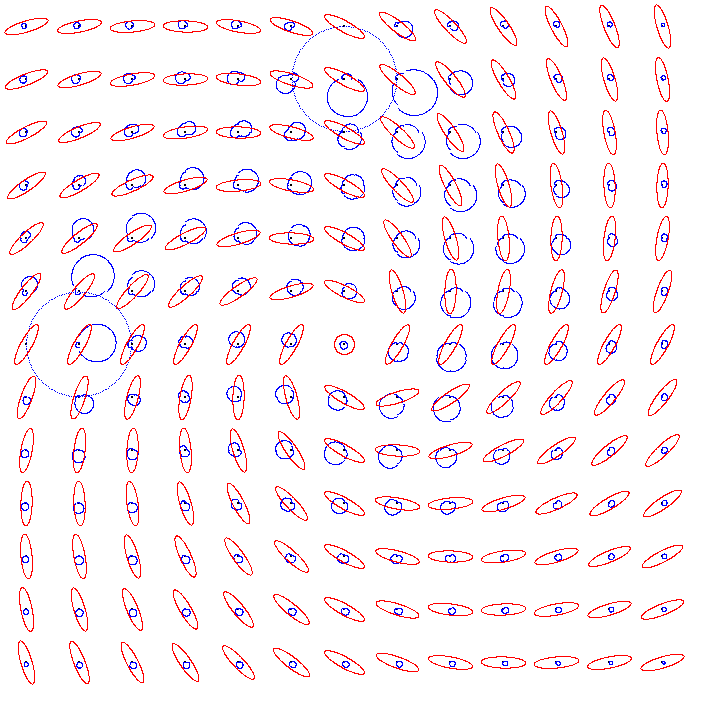
\includegraphics[width=0.9\textwidth]{img/spiral-two-dense.png}
    \label{a)}
	a)~two light sources
  \end{minipage}
  \begin{minipage}{0.4\textwidth}
    \centering
    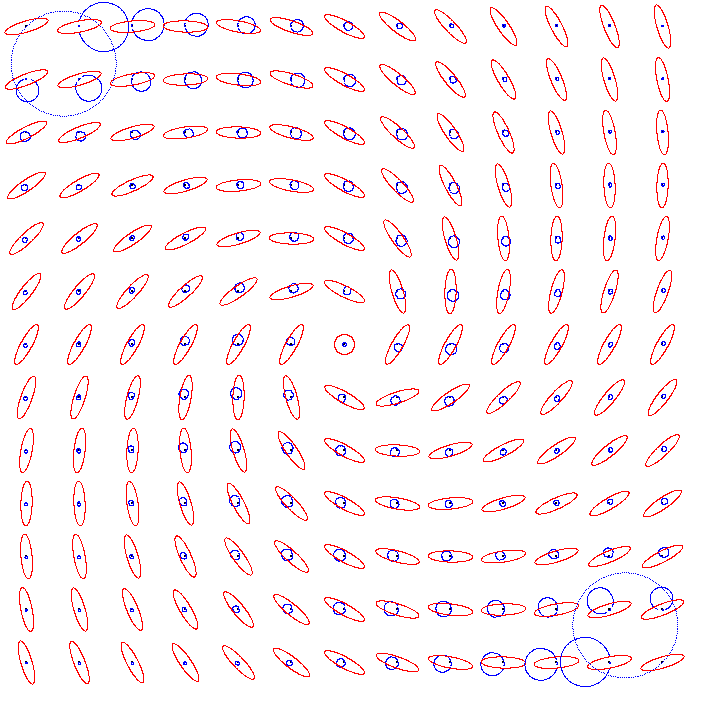
\includegraphics[width=0.9\textwidth]{img/spiral-two-wide.png}
    \label{b)}
	b)~symmetric light sources
  \end{minipage}
  \begin{minipage}{0.4\textwidth}
    \centering
    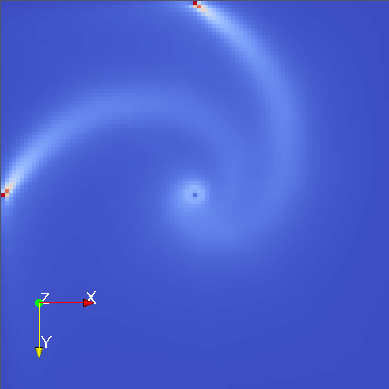
\includegraphics[width=0.9\textwidth]{img/spiral-temp2.png}
    \label{a)}
	c)~two light sources
  \end{minipage}
  \begin{minipage}{0.4\textwidth}
    \centering
    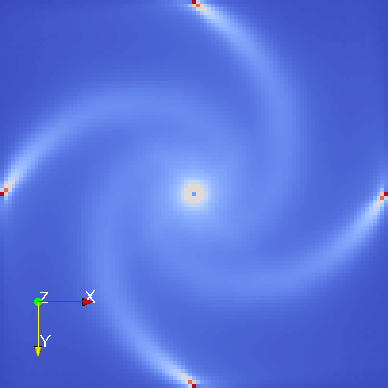
\includegraphics[width=0.9\textwidth]{img/spiral_full.png}
    \label{b)}
	d)~four light sources
  \end{minipage}
\caption{final light propagation distributions for ``spiral''-test field}
\label{spiral-tests}
\end{figure}
%%%%%%%%%%%%%%%%%%%%%%%%%%%%%%%%%%%%%%%%%%%%%%%%%%%%%%%%%%%%

% Alternative: put content in separate files
% Check the difference between including these files using \input{filename} and \include{filename} and see which one you like better
%\chapter{Einleitung}\label{intro}
%\input{introduction}
%
%\chapter{Voraussetzungen}\label{bg}
%\input{background}



\end{document}